%!TEX root = ../dokumentation.tex
\chapter{Backend}\label{ch:backend}
Als Backend wurde eine REST-API mit Node.js und dem Webframework Express entwickelt.

\section{Struktur}
Der Startpunkt des Backends ist die \hyperlink{https://github.com/Drinkler/Online-Shop/blob/master/backend/app.js}{app.js} Datei im Backend Ordner. Dort werden Daten initialisiert, Einstellungen vorgenommen, der Server mit der Datenbank verbunden und auch der Server gestartet.\\
Die eigentliche Struktur befindet sich im \hyperlink{https://github.com/Drinkler/Online-Shop/blob/master/backend/api}{api Ordner}. In diesem befindet sich eine \hyperlink{https://github.com/Drinkler/Online-Shop/blob/master/backend/api/index.js}{index.js} Datei. Diese Datei definiert alle Basisrouten für die API.\\
Die API ist in Controller, Middlewares, Models und Routes eingeteilt. 

\section{Validierung}
Zur Validierung der Request Bodies wurde das Modul \hyperlink{https://hapi.dev/module/joi/}{joi} verwendet. Es erleichtert die Validierung von Benuterdaten auf simpler, intuitiver und lesbarer Sprache.

\begin{lstlisting}[caption={Validierung des Sign ups (backend > api > middleware > validation.js)}]
const Joi = require("@hapi/joi");

const signUpValidation = (req, res, next) => {
    const signUpSchema = Joi.object({
        email: Joi.string().min(5).max(100).required().email(),
        name: Joi.string().alphanum().min(1).max(50).required(),
        surname: Joi.string().alphanum().min(1).max(50).required(),
        password: Joi.string().min(8).max(72).required(),
    });

    const { error } = signUpSchema.validate(req.body);
    if (error) return res.status(400).json({ error: error.details[0].message });

    next();
};
\end{lstlisting}

warum das schema nicht aussreicht
wie ein beispiel code aussieht.

\section{Authorisierung}

\section{Postman}
Postman ist ein API Entwicklungswerkzeug. Es bietet unter anderem die Möglichkeit HTTP Requests abzusenden und die dazugehörigen Responses anzuzeigen. Diese Funktionalität wurde, während der Entwicklung, verwendet um die Requests zu testen.\\
Alle Collections, Gruppierungen von Requests, und Umgebungsvariablen liegen im Postman Ordner. Diese können importiert werden.

\begin{figure}[H]
 \centering
 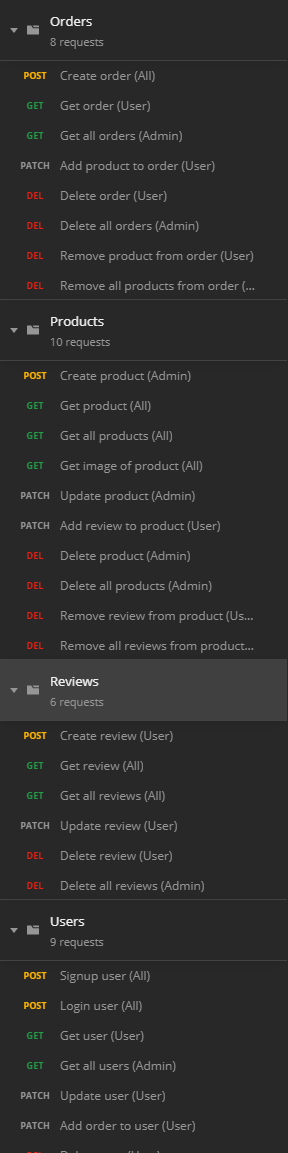
\includegraphics[width=\textwidth,height=0.6\textheight,keepaspectratio]{images/Postman_Collections.png}
 \caption{Collections in Postman}
 \label{fig:collections-postman}
\end{figure}

Abbildung \ref{fig:collections-postman} zeigt ein Teil der importieren Collections. Es gibt die Collections Orders, Products, Reviews und Users. Jede Collection enthält zugehörige Requests. Bei einem Request wird die HTTP Methode, sowie die Bennenung des Requests angezeigt. "(All)" bedeutet, dass keine Authorizierung benötigt wird. Für "(User)"  muss der Benutzer sich angemeldet haben und sein Token als Header mitversenden. Als "(Admin)" muss ein Token vorhanden sein, sowie in der Datenbank muss der Benutzer als Admin hinterlegt sein.\\
In Postman kann man einfach und Strukturiert seine Requests aufbauen. In den folgenden Abbildungen wird an dem Request "Create review (User)" die verschiedenen Hilfsmöglichkeiten gezeigt.

\begin{figure}[H]
 \centering
 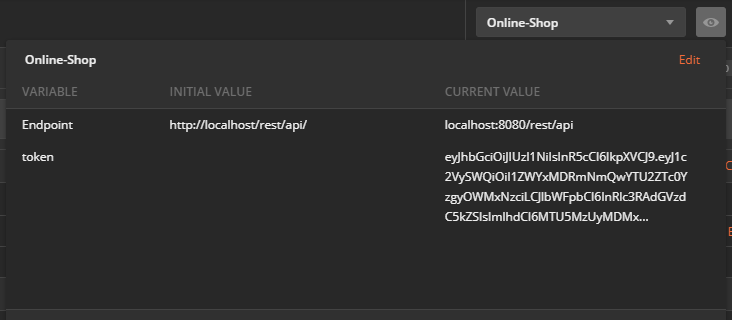
\includegraphics[width=0.8\textwidth,,keepaspectratio]{images/Postman_environment.png}
 \caption{Umgebungsvariablen in Postman}
 \label{fig:environment-postman}
\end{figure}

In Abbildung \ref{fig:environment-postman} werden die verwendeten Umgebungsvariablen gezeigt. Diese befinden sich oben rechts in Postman. Endpoint bestimmt den Basispfad der URL und token ist der Authorisierungstoken des Benutzers. Umgebungsvariablen werden mit doppelten geschweiften Klammern verwendet. Ein Beispiel dazu wäre in der Abbildung \ref{fig:authorization-postman} zu sehen.

\begin{figure}[H]
 \centering
 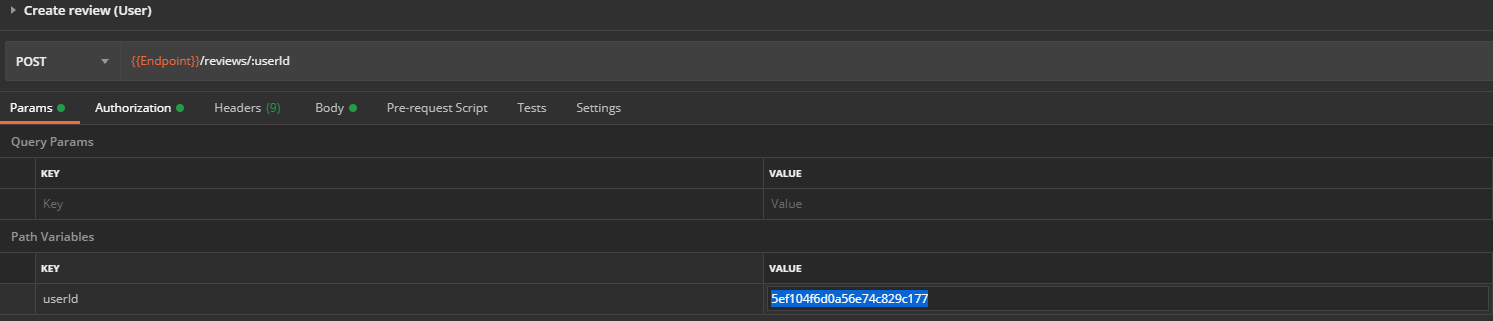
\includegraphics[width=0.9\textwidth,keepaspectratio]{images/Postman_params.png}
 \caption{Request Params in Postman}
 \label{fig:params-postman}
\end{figure}

Abbildung \ref{fig:params-postman} zeigt wie man Parameter bei einem Request eingeben kann. Dadurch muss man nicht die URL verändern, sondern kann bequem die Variablen in einer Tabelle anpassen. Parameter werden durch einen Doppelpunkt in Postman erkannt. In dieser Abbildung ist :userId ein Parameter. Dieser kann unter den Path Variables angepasst werden. Query Parameter sind Parameter die bei einem GET-Request nach dem Fragezeichen kommen.

\begin{figure}[H]
 \centering
 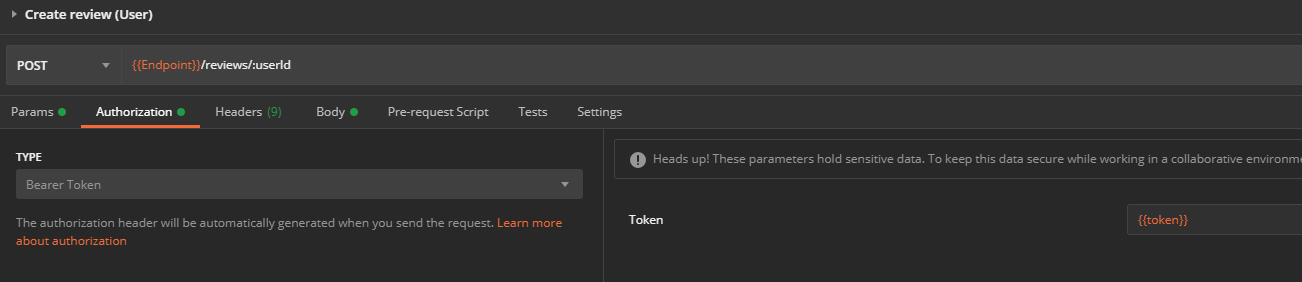
\includegraphics[width=\textwidth,height=0.6\textheight,keepaspectratio]{images/Postman_token.png}
 \caption{Request Authorization in Postman}
 \label{fig:authorization-postman}
\end{figure}

In Abbildung \ref{fig:authorization-postman} wird gezeigt wie man die Authorizierung eines Requestes festlegen kann. Im gesamten Projekt wird der Bearer Token verwendet. Diesen kann man unter TYPE festlegen. Als Token wird eine Variable definiert, dadurch muss man den Token nur einmal kopieren und als Umgebungsvariable festlegen. Den Token erhält man, sobald sich ein Benutzer anmeldet.

\begin{figure}[H]
 \centering
 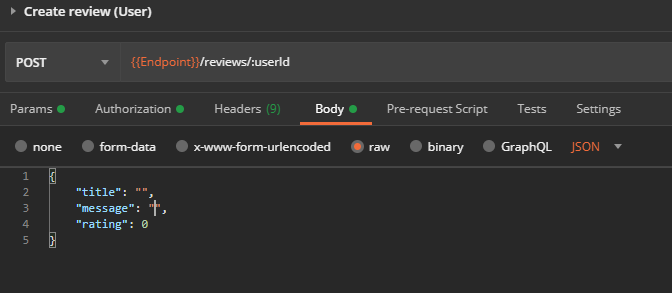
\includegraphics[width=0.75\textwidth,height=0.6\textheight,keepaspectratio]{images/Postman_body.png}
 \caption{Request Body in Postman}
 \label{fig:body-postman}
\end{figure}

Unter dem Reiter Body kann bei POST und PATCH Requests ein Inhalt mitversendet werden. Bis auf den "Create product (Admin)" Request ist der Body immer im JSON Format, siehe Abbildung \ref{fig:body-postman}.

\section{Swagger}
\hyperlink{https://swagger.io/}{Swagger} hilft bei der API-Entwicklung. Es bietet die Möglichkeit 

Wie es im Code aussieht
wie /rest/api/docs nachher aussieht.


